\documentclass[tikz]{standalone}

\usepackage{amsmath}
\usepackage{physics}

\usetikzlibrary{arrows.meta,backgrounds,fit,positioning}

\begin{document}
	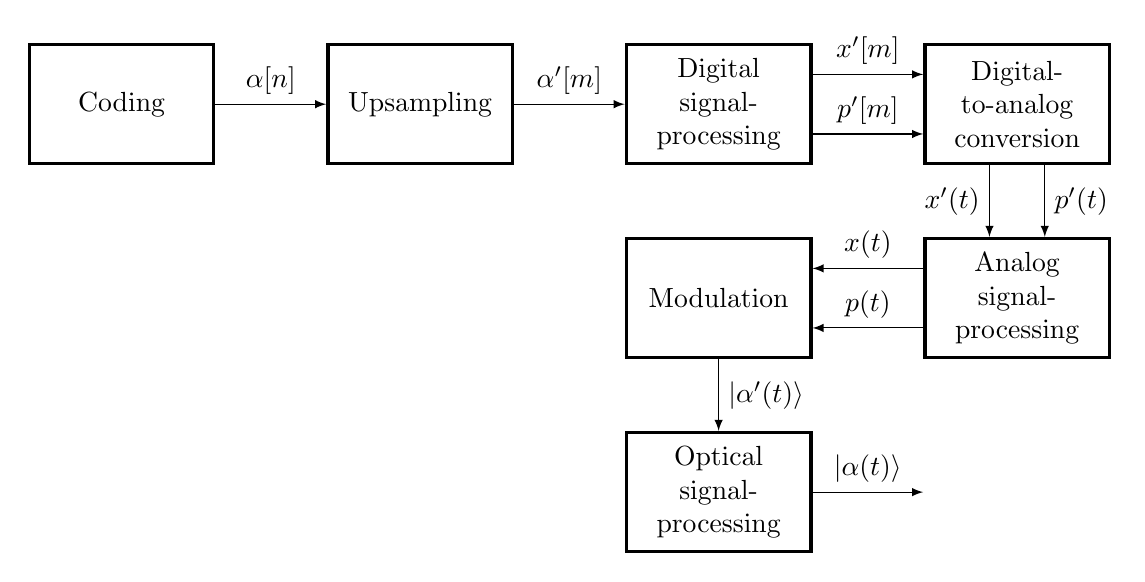
\begin{tikzpicture}[
		node distance=6ex and 4em,
		arrow/.style={-latex},
		block/.style={draw, very thick, fill=white, minimum height=10ex, minimum width=6em, text width=6em, align=center},
	]
		\coordinate (in) at (0,0);
		\node (cod) [block, right=of in] {Coding};
		\node (ups) [block, right=of cod] {Upsampling};
		\node (dsp) [block, right=of ups] {Digital signal-processing};
		\node (dac) [block, right=of dsp] {Digital-to-analog conversion};
		\node (asp) [block, below=of dac] {Analog signal-processing};
		\node (mod) [block, left=of asp] {Modulation};
		\node (osp) [block, below=of mod] {Optical signal-processing};
		\coordinate[right=of osp] (out);
		
		\draw[arrow] (cod) -- (ups) node[midway, above]{$\alpha[n]$};
		\draw[arrow] (ups) -- (dsp) node[midway, above]{$\alpha^\prime[m]$};
		\draw[arrow] ([yshift=2.5ex]dsp.east) -- ([yshift=2.5ex]dac.west) node[midway, above]{$x^\prime[m]$};
		\draw[arrow] ([yshift=-2.5ex]dsp.east) -- ([yshift=-2.5ex]dac.west) node[midway, above]{$p^\prime[m]$};
		\draw[arrow] ([xshift=-1em]dac.south) -- ([xshift=-1em]asp.north) node[midway, left]{$x^\prime(t)$};
		\draw[arrow] ([xshift=1em]dac.south) -- ([xshift=1em]asp.north) node[midway, right]{$p^\prime(t)$};
		\draw[arrow] ([yshift=2.5ex]asp.west) -- ([yshift=2.5ex]mod.east) node[midway, above]{$x(t)$};
		\draw[arrow] ([yshift=-2.5ex]asp.west) -- ([yshift=-2.5ex]mod.east) node[midway, above]{$p(t)$};
		\draw[arrow] (mod) -- (osp) node[midway, right]{$\ket{\alpha^\prime(t)}$};
		\draw[arrow] (osp) -- (out) node[midway, above]{$\ket{\alpha(t)}$};
	\end{tikzpicture}
\end{document}
